%%%%%%%%%%%%%%%%%%%%% chapter.tex %%%%%%%%%%%%%%%%%%%%%%%%%%%%%%%%%


\chapter{Wskaźniki analizy technicznej}
\label{Indicators} % Always give a unique label
% use \chaptermark{}
% to alter or adjust the chapter heading in the running head

W poniższym rozdziale zaprezentowane zostaną wskaźniki analizy technicznej oraz ich zastosowanie do handlu na wybranych parach walutowych, indeksach giełdowych i kontraktach terminowych.

\section{ROC --- wskaźnik Rate Of Change}
\label{sec:1ROC}
Rate Of Change, nazywany po polsku wskaźnikiem zmian, jest to wskaźnikiem który
mierzy procentową zmianę pomiędzy najnowszą ceną
zamknięcia a ceną $k$ okresów wcześniej. Sposób wyliczenia wartości wskaźnika ROC dla danego punktu w czasie przedstawiają wzory \ref{wzor_1} oraz \ref{wzor_2}.
\begin{equation}
ROC(\text{dziś}) = \frac{\text{Cena zamknięcia dziś} - \text{Cena zamknięcia } k \text{ okresów temu}}{\text{Cena zamknięcia } k \text{ okresów temu}}\\
\label{wzor_1}
\end{equation}
\begin{equation}
ROC(i) = \frac{C(i,4) - C(i-k,4)}{C(i-k,4)}
\label{wzor_2}
\end{equation}

\noindent Do podstawowych własności krzywej ROC należą:
\begin{itemize}
\item obrazuje ona jak zmieniała się cena obserwowanego rynku w danym okresie,
\item jeśli wartość oscylatora znajduje się poniżej zera, to obecna cena jest wyższa od tej sprzed $k$-godzin temu, analogicznie gdy oscylator znajduje się powyżej zera, oznacza to, że obecna cena jest niższa od tej sprzed $k$-godzin temu,
\item wzrastająca linia wskaźnika pokazuje, że różnice między
obecnym poziomem ceny a tym $k$ -czas temu się
zwiększają, malejąca mówi natomiast, że różnica ta się zmniejsza,
\item jeśli ceny akcji będą rosły to można oczekiwać, że linia
oscylatora będzie zachowywać się analogicznie, jeśli ceny będą natomiast malały to linia oscylatora powinna maleć.
\end{itemize}
Najważniejszą własnością opisywanego wskaźnika, stosowaną przy implementacjach strategii, jest fakt wskazywania momentów w których powinny zostać zawarte transakcje. Gdy wartość wskaźnika przetnie od dołu poziom zero to zakłada się, że jest to dobry moment kupna, jeśli przetnie poziom zera od góry to sprzedaży. Zostało to przedstawione na rysunku \ref{kupsprz}. \\
\begin{figure}[h!]
\centering
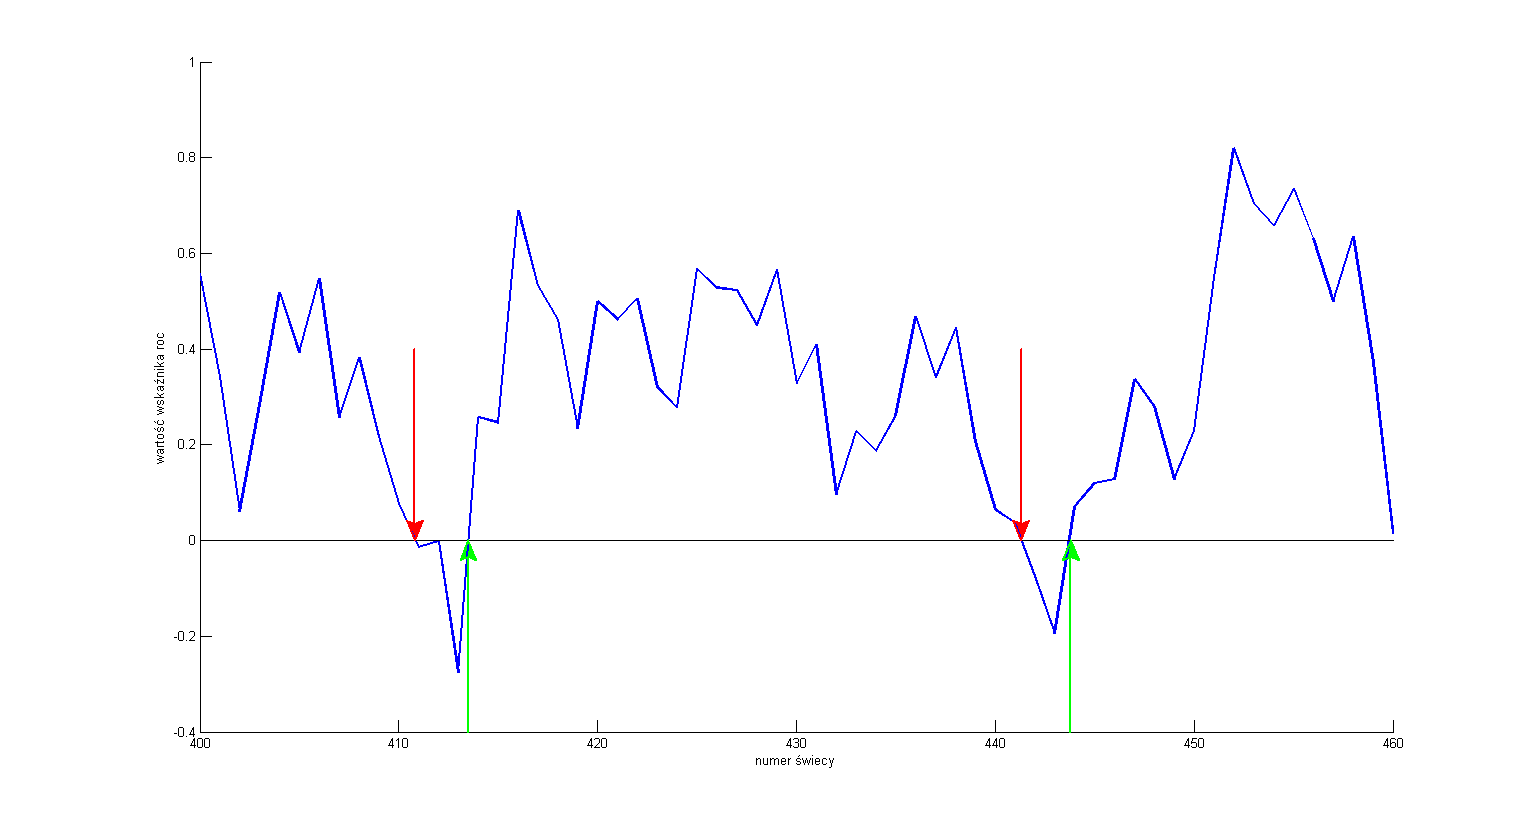
\includegraphics[width = \textwidth]{BuySell.png}
\caption{Fragment przykładowej krzywej ROC wraz z sygnałami kupna --- zielone strzałki oraz sygnałami sprzedaży --- czerwone strzałki}
\label{kupsprz}
\end{figure}
\FloatBarrier

\noindent Poniższy listing przedstawia zaimplementowaną strategię w środowisku MATLAB.
\begin{scriptsize}
\begin{lstlisting}
pocz = k+2;	
kon = size(C,1)-1;
iL = 0; % przekroczenie 0 w górę - kupno (L)
iS = 0; % przekroczenie 0 w dół - sprzedaż (S)
sumR = zeros(1,size(C,1));
R = zeros(1,size(C,1));
ROC_vec = zeros(1,kon-k+1);
ROC_vec(pocz-1) = ((C(pocz-1,4) - C(pocz-1-k,4))/C(pocz-1-k,4))*100;

recordReturn = 0;  % rekord zysku
recordDrawdown = 0;  % rekord obsuniecia
LastPos = 0;    % zmienna do przechowywania wartości na otwarciu ostatniej pozycji

for i=pocz:kon
    ROC_vec(i) = ((C(i,4) - C(i-k,4))/C(i-k,4))*100;  % obliczenie punktu krzywej ROC
    if ROC_vec(i)*ROC_vec(i-1)<=0   % przecięcie krzywej ROC z zerem
        if ROC_vec(i-1)<ROC_vec(i)  % warunek kupna
            if iL+iS>0
                R(i) = -C(i+1,4)+LastPos-spread;   % zamknięcie S
            end
            LastPos = C(i+1,1);   % otworzenie L
            iL = iL + 1;
        elseif ROC_vec(i-1)>ROC_vec(i)  % warunek sprzedaży
            if iL+iS>0
                R(i) = C(i+1,4)-LastPos-spread;  % zamknięcie L
            end
            LastPos = C(i+1,1);   % otworzenie S
            iS = iS + 1;
        end
    end
    sumR(i) = sum(R(pocz:i));
  
    if sumR(i)>recordReturn
        recordReturn=sumR(i);
    end
    
    if sumR(i)-recordReturn<recordDrawdown
        recordDrawdown=sumR(i)-recordReturn;  
    end

end

Calmar=-sumR(kon)/recordDrawdown;
profit = sumR(kon);

end
\end{lstlisting}
\end{scriptsize}


Na podstawie zebranych informacji dotyczących wskaźnika $ROC$ utworzono prostą strategię inwestycyjną bazującą na regule: jeśli linia $ROC$ przetnie się z poziomem zera od dołu, to otwierana jest pozycja długa ($L$), a zamykana pozycja krótka ($S$), która została wcześniej otwarta. Gdy natomiast nastąpi przecięcie linii $ROC$ z poziomem zera od góry to otwarta zostanie pozycja krótka, a zamknięta długa. Badania zostały przeprowadzone na parze walutowej $EURJPY$ (szereg czasowy przedstawiony na rysunku \ref{rysunek2}). \\
\begin{figure}[h!]
\centering
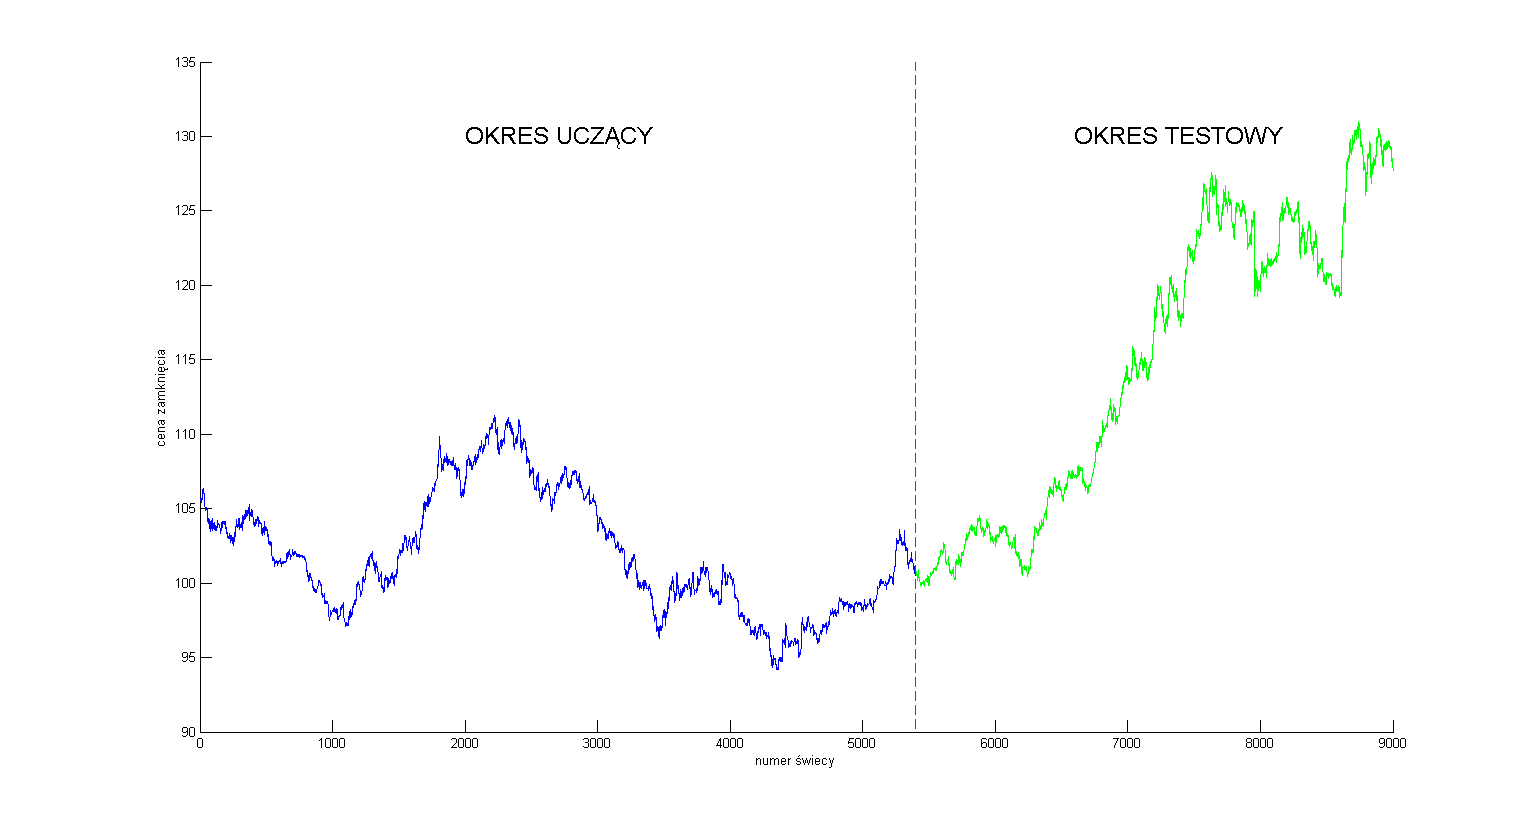
\includegraphics[width = \textwidth]{podzialDanych.png}
\caption{Badany szereg czasowy z podziałem na część uczącą i testową}
\label{rysunek2}
\end{figure}
\FloatBarrier
Cały zbiór danych (świec) podzielony został na dwie części: uczącą ($60\%$ całości) oraz testową ($40\%$ całości). W przeprowadzonych badaniach poszukiwano optymalnej wartości parametru $k$ na okresie uczącym, następnie weryfikowano otrzymane wyniki na okresie testowym. Wybór optymalnej wartości parametru $k$ determinowano na dwa sposoby:
\begin{itemize}
\item otrzymanego zysku skumulowanego,
\item wskaźnika Calamara.
\end{itemize}

\noindent \textbf{I Wyniki badań przy maksymalizacji po zysku.}\\
\begin{figure}[h!]
\centering
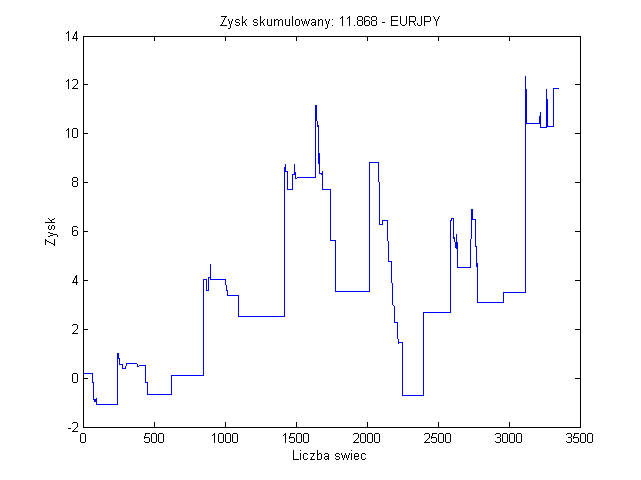
\includegraphics[width = 0.6\textwidth]{ROC_EURJPY_LS_SearchBestK_zysk.png}
\caption{Zysk skumulowany EURJPY na okresie testowym przy maksymalizacji według zysku}
\end{figure}
\FloatBarrier
\begin{verbatim}
OKRES UCZĄCY
Długość cyklu: 	89
Zysk skumulowany: 	16.81
Calmar: 	2.66
Liczba otwartych pozycji długich: 	100
Liczba otwartych pozycji krótkich: 	100

OKRES WALIDUJĄCY
Długość cyklu: 	89
Zysk skumulowany: 	11.87
Calmar: 	1.00
Liczba otwartych pozycji długich: 	61
Liczba otwartych pozycji krótkich: 	61
\end{verbatim}
\newpage
\textbf{II Wyniki badań przy maksymalizacji po wskaźniku Calmara.}\\
\begin{figure}[h!]
\centering
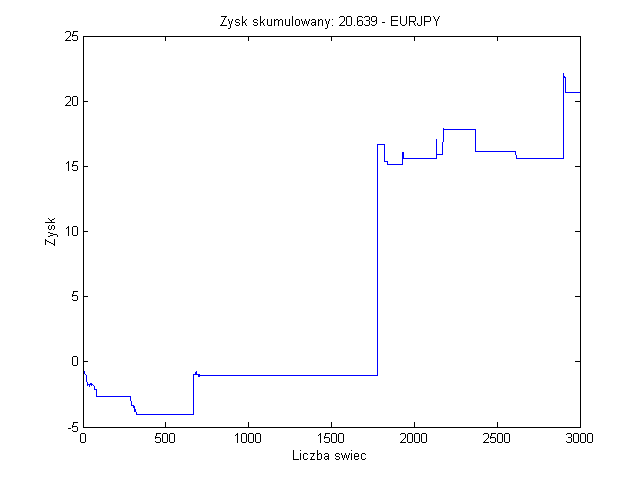
\includegraphics[width = 0.6\textwidth]{ROC_EURJPY_LS_SearchBestKCalmar_zysk.png}
\caption{Zysk skumulowany EURJPY na okresie testowym przy maksymalizacji według Calmara}
\end{figure}
\FloatBarrier
\begin{verbatim}
OKRES UCZĄCY
Długość cyklu: 	230
Zysk skumulowany: 	12.82
Calmar: 	3.83
Liczba otwartych pozycji długich: 	52
Liczba otwartych pozycji krótkich: 	51

OKRES TESTUJĄCY
Długość cyklu: 	230
Zysk skumulowany: 	20.64
Calmar: 	5.08
Liczba otwartych pozycji długich: 	28
Liczba otwartych pozycji krótkich: 	29
\end{verbatim}
%
